% !TEX root = ../main.tex

\chapter{基于享乐联盟博弈的分布式任务分配}
\label{chap:hedonic}

\section{引言}
\label{hg:sec:intro}

使用享乐联盟博弈模型(Hedonic Coalition Game, HCG)解决任务分配问题的思路是将任务分配问题看作是智能体划分问题,按照任务或目标的不同划分联盟,每个智能体对不同联盟有着不同的偏好,智能体会根据自己的偏好选择自己的联盟,最终所有智能体在确定了自己的所属联盟后,便得到了任务分配的解。本章将建立基于HCG的任务分配框架并提出对应求解算法,并通过仿真对比实验验证其有效性、


% ---------------------
% ---------------------
\section{享乐联盟博弈模型}
\label{hg:sec:hgmodel}

在介绍HCG模型概念之前,需要先在第\ref{chap:model}章建立的模型的基础上进行一些修正。沿用第\ref{chap:model}章中的符号和定义,智能体集合为$\mathcal{M}=\{\mathcal{M}_1,\dots,\mathcal{M}_{n_m}\}$,任务集合为$\mathcal{T} = \{\mathcal{T}_0,\mathcal{T}_1,\dots,\mathcal{T}_{n_t}\}$。在此章中,不再使用任务效用函数概念,而每个智能体拥有一个智能体效用函数,因此可将智能体效用函数简记为$U_i(\mathcal{T}_j,p):\mathcal{T} \times |\mathcal{M}| \mapsto \mathbb{R}$,这里的智能体效用函数与第\ref{chap:pg}章中使用WLU定义的智能体效用函数不同,除了与当前分配的任务$\mathcal{T}_j$有关外,还与同时选择该任务的智能体个数$p$有关。对于$\mathcal{T}_0$,定义$U_i(\mathcal{T}_0,n)=0,\forall \mathcal{M}_i \in \mathcal{M}, 0 \leq n \leq n_m$。设当前分配解为$a=(a_1,a_2,\dots,a_{n_m})$,全局效用函数被定义为

\begin{equation}
\label{hcg:eq:gloablU}
	U_g(a) = \sum_{a_i \in a} U_i(a_i,p_j),
\end{equation}
其中
\begin{equation}
\label{hcg:eq:parcitipants}
	p_j = \sum_{a_i \in a} I\{a_i = \mathcal{T}_j\},\ \mathcal{T}_j \in \mathcal{T}.
\end{equation}

为了建立HCG模型,现引入如下概念。

\begin{definition}[偏好关系]
	对于每个智能体$\mathcal{M}_i$,将二元组$x=(\mathcal{T}_j,p)$称为一组联盟对,意味着“智能体$\mathcal{M}_i$将与$p$个队友一起执行任务$\mathcal{T}_j$”,记所有联盟对集合为$\mathcal{X}=\mathcal{T}\times\{1,\dots,n_m\}$。在所有联盟对上定义一个关于效用的偏序关系$\succ_i$,对任意$x_1,x_2 \in \mathcal{X}$,$x_1 \succ_i x_2$意味着智能体$\mathcal{M}_i$对联盟对$x_1$有较强的偏好,此外还可定义$x_1 \sim_i x_2$为智能体$\mathcal{M}_i$对$x_1$和$x_2$的偏好无差别,$x_1 \succeq_i x_2$意味着智能体$\mathcal{M}_i$对联盟对$x_1$有较弱的偏好。
\end{definition}

结合之前定义的智能体效用函数,偏好关系$\succ_i$可以定义为
\begin{equation}
\label{hcg:eq:preference}
	(\mathcal{T}_1,p_1) \succ_i (\mathcal{T}_2,p_2),\quad \text{if}\ U_i(\mathcal{T}_1,p_1) > U_i(\mathcal{T}_2,p_2).
\end{equation}

HCG模型$\mathcal{G}=(\mathcal{M},\mathcal{T},\succeq_i)$是由智能体集合,任务集合和智能体的偏好关系组成的博弈模型。在HCG模型框架下解决任务分配问题,实质上是将任务分配问题看做是对智能体的分组问题,智能体可根据自己的偏好自行选择加入某个联盟小组,当所有智能体确定自己的联盟后,即可得到一组任务分配方案。下面的定义是对智能体联盟和HCG模型中的纳什均衡进行介绍。


\begin{definition}[联盟划分]
	对于HCG模型$\mathcal{G}$,定义一个集合$\Pi = \{S_0,S_1,\dots,S_{n_t}\}$,其中元素联盟集合$S_j \subseteq \mathcal{M},j=1,\dots,n_m$为同时选择任务$\mathcal{T}_j$的所有智能体集合,特别地,$S_0$代表该智能体没有选择任何任务。由于每个智能体智能选择一个任务,因此$\cup_{j=0}^{n_t} S_j = \mathcal{M},\ S_i \cap S_j =\emptyset,\ i \neq j$。为了后续论述方便,用$\Pi(i)$表示智能体$\mathcal{M}_i$选择的任务序号,用$S_{\Pi(i)}$表示智能体$\mathcal{M}_i$所属的联盟集合,即$S_{\Pi(i)}=\{S_j \in \Pi|\mathcal{M}_i \in S_j\}$。
\end{definition}


\begin{definition}[HCG模型的纳什均衡]
	当在划分$\Pi$下,对于任意智能体$\mathcal{M}_i \in \mathcal{A}$都有
	\begin{equation}
	\label{hcg:eq:nash_stable}
		(t_{\Pi(i)},|S_{\Pi(i)}|) \succeq_i (t_j,|S_j \cup \{a_i\}|),\quad \forall S_j \in \Pi,
	\end{equation}
	则划分$\Pi$被称为是纳什均衡划分.
\end{definition}

因此,在联盟的概念下,HCG模型的纳什均衡状态意味着每个智能体均根据自身的效用函数选择自己最“喜爱”的联盟,在此状态下,所有智能体不会产生离开当前联盟的动力,此时也就得到了任务分配的稳定方案。



% ------------------------------------
% ------------------------------------
\section{基于享乐联盟博弈模型设计}
\label{hcg:HGTA}

\subsection{智能体效用函数设计}
\label{hcg:coalition}

为了保证HCG模型纳什均衡状态存在的必然性,需要对智能体效用函数$U_i(\mathcal{T}_j,p)$做出一定的要求。

\begin{definition}[社交疏远性质]
\label{hcg:eq:spao}
	如果智能体的偏好关系满足对任意任务$\mathcal{T}_j \in \mathcal{T} \setminus \{\mathcal{T}_0\}$,
	\begin{equation}
	\label{hcg:eq:spaoPrefer}
		(\mathcal{T}_j,p_1) \succeq_i (\mathcal{T}_j,p_2),\quad p_1 < p_2,\ p_1,p_2 \in \{1,\dots,n_m\},
	\end{equation}
	即智能体效用随着同联盟的成员数量增加而递减,则称该智能体具有社交疏远性质(Social Inhibition Characteristic, SIC)。若使用式(\ref{hcg:eq:preference})的定义,则SIC表现在智能体效用函数上为
	\begin{equation}
	\label{hcg:eq:spaoU}
		U_i(\mathcal{T}_j,p_1) > U_i(\mathcal{T}_j,p_2),\quad p_1<p_2,\ p_1,p_2 \in \{1,\dots,n_m\}.
	\end{equation}
\end{definition}

带有SIC的智能体组成的HCG模型一定存在纳什均衡。事实上有如下定理。

\begin{theorem}
	设HCG模型$\mathcal{G}=(\mathcal{M},\mathcal{T},\succeq_i)$中的智能体都具有SIC,则该模型一定存在纳什均衡。
	\begin{proof}
		可使用数学归纳法证明。当智能体数量$n_m=1$时,定理显然成立。
		
		假设$n_m=k$时,定理成立,即模型$\mathcal{G}=(\mathcal{M},\mathcal{T},\succeq_i)$存在纳什均衡。则当$n_m=k+1$时,新模型为$\widetilde{\mathcal{G}}=(\widetilde{\mathcal{M}},\mathcal{T},\succeq_i)$。设$\mathcal{M}_r \in \widetilde{\mathcal{M}}, \mathcal{M}_r \notin \mathcal{M}$,则$\widetilde{\mathcal{M}}=\mathcal{M} \cup \{\mathcal{M}_r\}$。
		
		对一个联盟划分$\Pi$,和任意的智能体$\mathcal{M}_i$,定义联盟可容纳额外成员数$\Delta_{\Pi(i)}$为当前联盟在不会使智能体$\mathcal{M}_i$不选择其他联盟的情况下,可额外增加的最大智能体个数,即
		\begin{equation}
		\label{hcg:eq:maxDelta}
			\Delta_{\Pi(i)}:= \min_{S_j \in \Pi \setminus \{S_{\Pi(i)}\}} \max_{\Delta \in \mathbb{Z}}\{\Delta|(\mathcal{T}_{\Pi(i)},|S_{\Pi(i)}|+\Delta) \succeq_i (\mathcal{T}_j, |S_j \cup \{\mathcal{M}_i\}|) \}.
		\end{equation}
		
		由SIC定义可知,$\Delta_{\Pi(i)}$满足以下性质:(1)如果划分$\Pi$是纳什均衡的,则对于任意智能体$\mathcal{M}_i$,有$\Delta_{\Pi(i)}\geq 0$;(2)如果$\Delta_{\Pi(i)}<0$,则智能体$\mathcal{M}_i$会选择离开当前联盟;(3)智能体$\mathcal{M}_i$在更换联盟后,设新联盟划分为$\Pi'$,则有$\Delta_{\Pi'(i)} \geq 0$。
		
		设$\Pi_0$是博弈$\mathcal{G}$的一个纳什均衡。当智能体$\mathcal{M}_r$选择了一个任务之后,会形成一个新的联盟划分$\Pi_1$,由第(3)点性质可知,$\Delta_{\Pi_1(r)}\geq 0$。此时若不存在智能体$\mathcal{M}_q \in \mathcal{A}$,使得$\Delta_{\Pi_1(q)}<0$,则可知划分$\Pi_1$是一个纳什均衡。
		
		假设此时至少存在一个智能体$\mathcal{M}_q$满足$\Delta_{\Pi_1(q)}<0$,则该智能体必定在$\mathcal{M}_r$所在的联盟中。由于此时智能体$\mathcal{M}_q$会选择另一个联盟加入,并再次形成一个新的联盟划分$\Pi_2$,因此此时智能体$\mathcal{M}_r$满足$\Delta_{\Pi_2(r)} \geq 1$(因为在$\mathcal{M}_q$移动之前已经满足不小于0)。换句话说,此时$\mathcal{M}_r$将不会再改变自己的联盟,即使其他智能体不断的变换自己的联盟。这意味着至多经过$|\widetilde{\mathcal{M}}|$次迭代,在最终的划分$\widetilde{\Pi}$下,所有的智能体都会满足$\Delta_{\widetilde{\Pi}(i)}\geq 0$,因此$\widetilde{\Pi}$是一个纳什均衡。
		
		由于定理在$n_m=k+1$时成立,因此归纳可得原定理成立。
	\end{proof}
\end{theorem}

根据以上定理,结合第\ref{chap:model}章中的效用函数定义,定义本章使用的智能体效用函数为

\begin{equation}
\label{hcg:eq:agentU}
	U_i(\mathcal{T}_j,p) = \frac{r(\mathcal{T}_j,|S_j|)}{|S_j|} - c_i(\mathcal{T}_j)
\end{equation}

其中$r(\mathcal{T}_j,|S_j|)$为导弹和联盟成员一起攻击目标$\mathcal{T}_j$可获得的回报,并假设联盟所有成员平分任务回报。在空战场景中,攻击同一个目标的导弹数量越多,击中的目标的概率越大,但当数量超过一定界限时,再增加导弹数量对于目标的攻击起到的作用很小,即随着联盟成员的数量增加,导弹所得到的边际回报在递减。因此可定义任务回报函数$r(\mathcal{T}_j,|S_j|)$为

\begin{equation}
\label{hcg:eq:task_reward}
	r(\mathcal{T}_j,|S_j|) = r_j^{\text{min}} \cdot \log_{\varepsilon_j} (|S_j|+\varepsilon_j-1),
\end{equation}
其中$r_j^{\text{min}}$代表联盟中只有一位成员时的回报值,$\varepsilon_j>0$是一个正数,与边际回报的递减速率有关。该函数的图像如图\ref{hcg:fig:rewardfunc}(a)所示,图中$r_j^{\text{min}}=10, \varepsilon_j = 3$。将任务回报函数代入式(\ref{hcg:eq:agentU})可得智能体效用函数为

\begin{equation}
\label{hcg:eq:agentU_reward}
	U_i(\mathcal{T}_j,|S_j|) = \frac{r_j^{\text{min}} \cdot \log_{\varepsilon_j} (|S_j|+\varepsilon_j-1)}{|S_j|} - c_i(\mathcal{T}_j),
\end{equation}
智能体效用函数的图像如图\ref{hcg:fig:rewardfunc}(b)所示,由图像可知,该智能体效用符合SIC要求。

\begin{figure}[!hbtp]
  \centering
  \bisubcaptionbox{任务回报函数}%
                  {Task Reward Function}%
                  {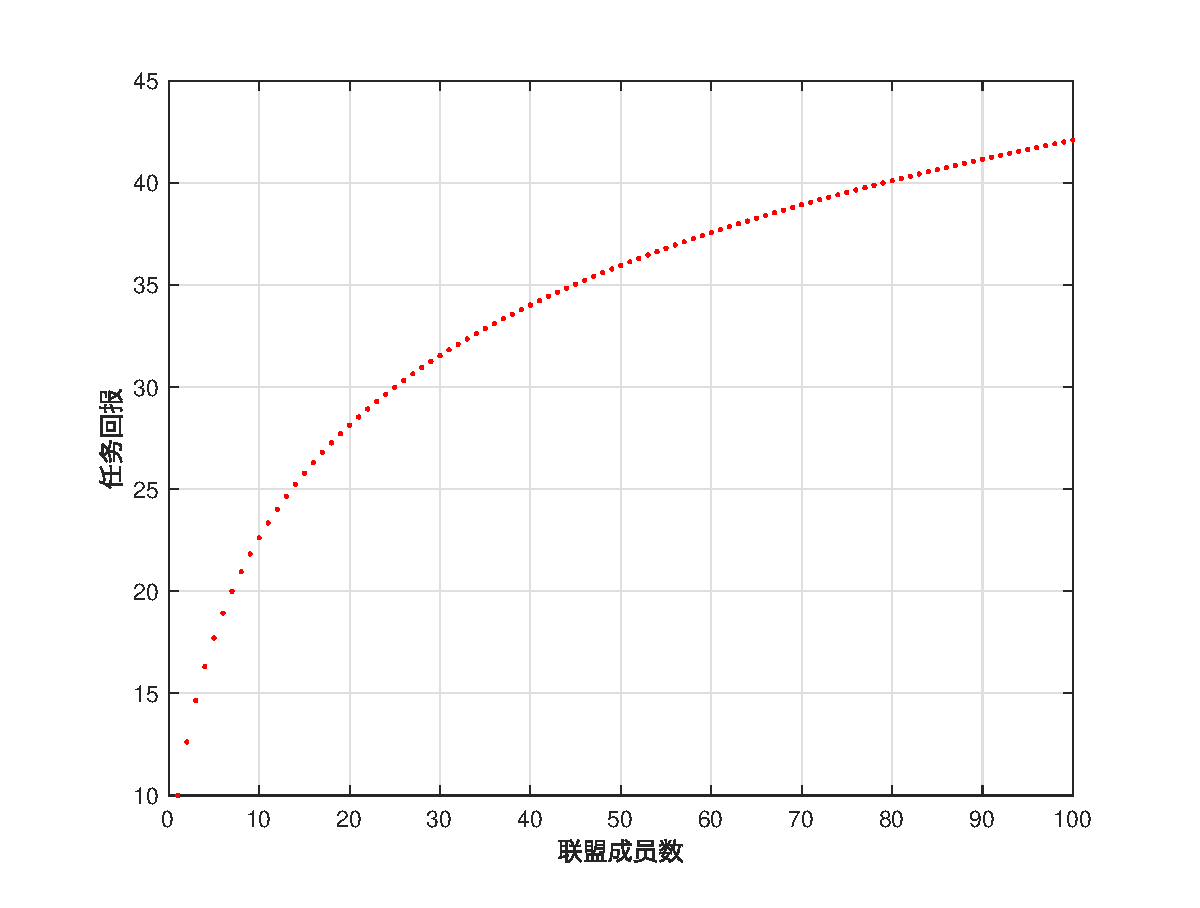
\includegraphics[scale=0.3]{taskreward.eps}}
  \hspace{2cm}
  \bisubcaptionbox{智能体回报函数}%
                  {Agent Reward Function}%
                  {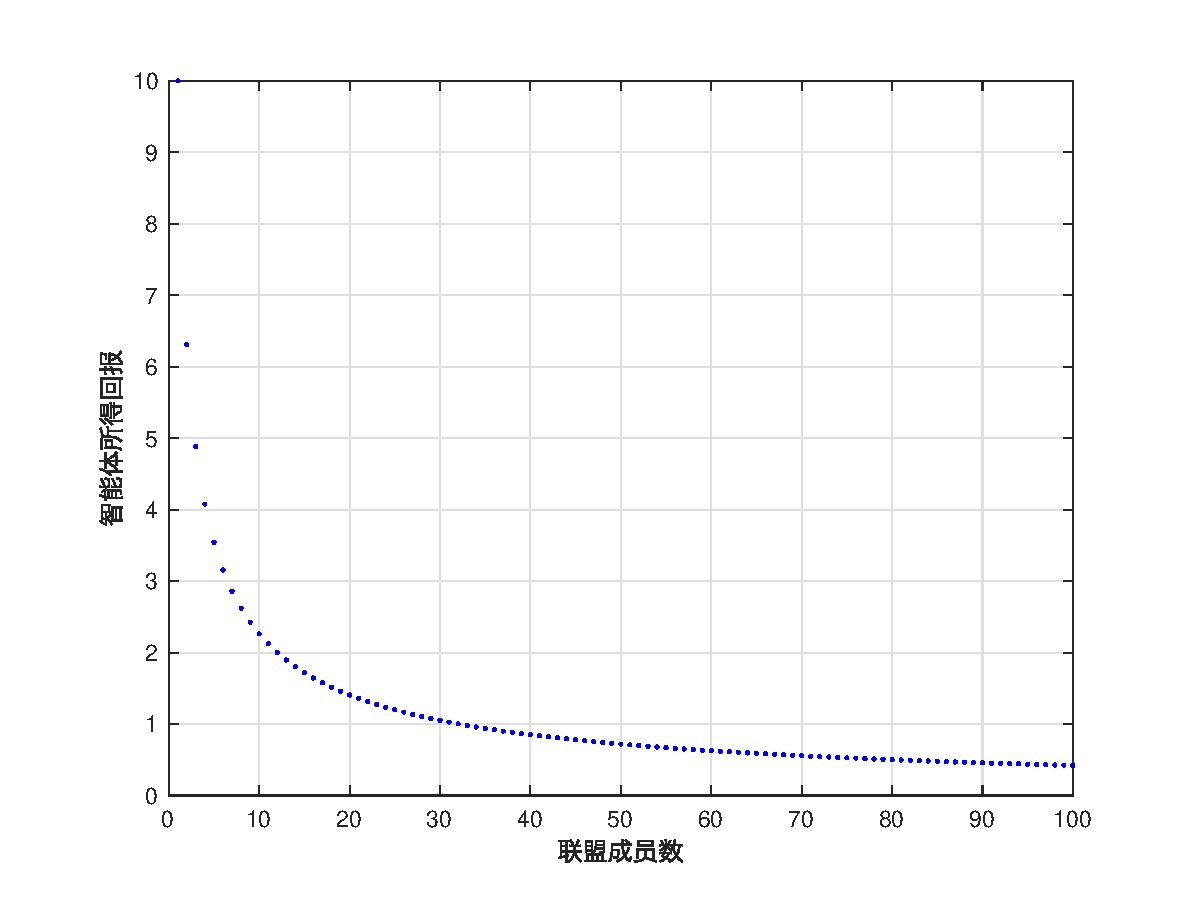
\includegraphics[scale=0.3]{agentreward.eps}}
  \bicaption{HCG模型的回报函数}
            {Reward Function of HCG Model}
  \label{hcg:fig:rewardfunc}
\end{figure}

与第\ref{chap:pg}章中遇到的约束条件处理问题类似,在本章使用HCG模型的场景中,需要限定得到的联盟划分满足约束条件式(\ref{model:eq:bmax})。由于本节定义的智能体效用函数与联盟成员数有关,而约束条件也是对于执行同一任务的智能体个数的限定,因此可以直接对智能体效用函数进行进一步改进,使得智能体在加入一个联盟时,会考虑到加入该联盟后该联盟成员数是否仍满足约束条件。如果加入该联盟后约束条件不再满足,则智能体不会选择加入该联盟。具体来说,引入改进智能体效用函数$\widetilde U_i(\mathcal{T}_j,|S_j|)$为

\begin{equation}
\label{hcg:eq:modifiedAgentU}
	\widetilde U_i(\mathcal{T}_j,|S_j|) = 
	\begin{cases}
		U_i(\mathcal{T}_j,|S_j|),\ & \text{if $|S_j|\leq b_{\text{max}}^{(j)}$,}\\
		0,\ & \text{otherwise}
	\end{cases}
\end{equation}

当智能体即将选择加入的联盟已经达到约束边界时,若智能体加入,则得到的效用将会是0,因此智能体最终不会选择再加入该联盟,从而保证了求解的可行性。

%---------------------------
%---------------------------
\section{基于享乐联盟博弈模型的决策算法}
\label{hcg:decision}

\subsection{SAP算法}
在HCG模型下的智能体决策算法仍可使用第\ref{chap:pg}章\ref{pg:pgta:protocal}节中使用的几种决策算法,本节选择使用SAP算法,下面算法\ref{hcg:algo:HCGSAP}将直接给出使用SAP的HCG决策算法流程。

\begin{algorithm}[htb]
	\caption{使用SAP的HCG决策算法流程}
	\label{hcg:algo:HCGSAP}
	\small
	\SetAlgoLined
	\KwIn{$\mathcal{M},\mathcal{T},\mathcal{A},r$}
	\KwOut{均衡解$a^*$}
	\tcp{初始化参数}
	$k \gets 1$\;
	随机生成任务分配初始解$a(0)$\;
	\tcp{计算初始每个任务联盟的成员数}
	$\text{CoWorkerNums}_j(0) \gets \sum_{\mathcal{M}_i \in \mathcal{M}} I\{a_i(0)=\mathcal{T}_j\}$\;
	\While{true}{
		随机选择一个智能体$\mathcal{M}_i$\;
		$n_i=|\mathcal{A}_i|$\;
		\For{$j=1:n_t$}{
			根据式(\ref{hcg:eq:agentU_reward})计算$U_i(\mathcal{T}_j,|S_j|+1)$\;
		}
		根据式(\ref{pg:eq:sappdf})计算$p_i(k)$\;
		根据$p_i(k)$随机选择任务$\mathcal{T}_l$\;
		\tcp{更新联盟划分和联盟成员数}
		$a_i(k) \gets  \mathcal{T}_l$\;
		$\text{CoWorkerNums}_{a_i(k-1)}(k) \gets \text{CoWorkerNums}_{a_i(k-1)}(k) - 1$\;
		$\text{CoWorkerNums}_{a_i(k)}(k) \gets \text{CoWorkerNums}_{a_i(k)}(k) + 1$\;
		$k\gets k+1$\;
	}
\end{algorithm}

%----------------------------
\subsection{分布式互斥算法}

本节将提出HCG模型下的另一种决策算法,称为互斥算法(Mutual Exclusion Algorithm, MEA)。MEA在每次迭代中,所有智能体都会做出自己的决策,但智能体在交互中会只保留一个智能体的决策结果。算法\ref{hcg:algo:decsion}和算法\ref{hcg:algo:dmea}给出了使用MEA的分布式决策算法,其中算法\ref{hcg:algo:decsion}是智能体$\mathcal{M}_i$在每次迭代的决策过程,算法\ref{hcg:algo:dmea}是MEA的实现。

\begin{algorithm}[htb]
	\caption{智能体$\mathcal{M}_i$的决策算法流程}
	\label{hcg:algo:decsion}
	\small
	\SetAlgoLined
	\KwIn{$\mathcal{M},\mathcal{T},\mathcal{A},r$}
	\KwOut{联盟划分$\Pi$}
	\tcp{初始化参数}
	$\text{satisfied} \gets false$\;
	$\text{evolved}^i\gets 0$;\tcp{智能体更新决策次数}
	$\text{stamp}^i \gets 0$;\tcp{时间戳}
	$\Pi^i \gets \{S_0=\mathcal{M},S_j=\emptyset, \forall \mathcal{T}_j \in \mathcal{T} \}$\;
	\While{true}{
		\tcp{每次迭代智能体做出新决策}
		\If{$\text{satisfied}=false$}{
			$(\mathcal{T}_{j^*},|S_{j^*}|) \gets \arg \max_{S_j \in \Pi^i} U_i(\mathcal{T}_j,|S_j \cup \{\mathcal{M}_i\}|)$\;
			\If{$(\mathcal{T}_{j^*},|S_{j^*}|)\succ_i (\mathcal{T}_{\Pi^i(i)},|S_{\Pi^i(i)}|)$}{
				智能体$\mathcal{M}_i$加入$S_{j^*}$,更新划分$\Pi^i$\;
				$\text{evolved}^i \gets \text{evolved}^i+1$\;
				$\text{stamp}^i \gets \mathrm{rand}[0,1]$\;
			}
		$\text{satisfied}\gets true$\;
		}
	智能体$\mathcal{M}_i$向邻居发送信息$I^i=\{\text{evolved}^i,\text{stamp}^i,\Pi^i\}$,并从其邻居节点获取信息$I^k,\forall \mathcal{M}_k \in \mathcal{N}_i$\;
	构造信息集$\mathcal{I}^i=\{I^i\}\cup\{I^k,\forall \mathcal{M}_k \in \mathcal{N}_i\}$\;
	\tcp{运行互斥算法}
	$\{\text{evolved}^i,\text{stamp}^i,\Pi^i\}, \text{satisfied} \gets \text{DMEA}(\mathcal{T}^i)$\;
	}
	
\end{algorithm}

\begin{algorithm}[htb]
	\caption{分布式互斥算法(DMEA)}
	\label{hcg:algo:dmea}
	\small
	\SetAlgoLined
	\KwIn{$\mathcal{I}^i$}
	\KwOut{$\{\text{evolved}^i,\text{stamp}^i,\Pi^i\},\text{satisfied}$}
	\tcp{初始化参数}
	$\text{satisfied} \gets true$\;
	\For{$M_k \in \mathcal{M}^i$}{
		\If{$\text{evolved}^k>\text{evolved}^i)\ \text{or}\ (\text{evolved}^k=\text{evolved}^i\ \text{and}\ \text{stamp}^k > \text{stamp}^i)$}{
			$\text{evolved}^i \gets \text{evolved}^k$\;
			$\text{stamp}^i \gets \text{stamp}^k$\;
			$\Pi^i \gets \Pi^k$\;
			$\text{satisfied} \gets false$\;
		}
	}
\end{algorithm}

每个智能体在决策过程中都有自己的划分方式$\Pi^i$;变量satisfied是一个布尔变量,用于表示智能体是否对当前划分$\Pi^i$满意,即不会离开当前联盟;$r^i \in \mathbb{N}$是表示智能体做出了新决策,改变了联盟划分的次数;$s^i \in [0,1]$是一个服从0到1之间平均分布的随机变量,它会在划分$\Pi$每次更新时被生成,作用是作为一种时间戳,用于在后续交互时提供一致的依据。智能体在每次迭代中的决策过程是这样的:首先根据当前已知的划分$\Pi^i$,检查在该划分下,假设其他智能体不改变联盟,找出自己加入哪个联盟会得到最高效用(算法\ref{hcg:algo:decsion}第7行)。如果加入该联盟所得效用比自己当前联盟可得到的效用更高,则智能体会选择加入新联盟,同时增价更新次数$r^i$,并随机生成一个时间戳$s^i$(算法\ref{hcg:algo:decsion}第8-11行)。

由于每个智能体存储的都是自己的划分方式,因此在进行交互协商时,为了达成一致,只能有一种划分方式被广泛接受,称这个划分方式为有效划分。算法\ref{hcg:algo:dmea})介绍的MEA使得智能体能够在局部通信的情况下获得有效划分。智能体交互时传递的信息集为$I^i=\{\text{evolved}^i,\text{stamp}^i,\Pi^i\}$,包括自己的划分方式,划分更新次数和更新时间戳。在交互时,更新次数更多的划分方式被认为更加有效,如果更新次数一样,则选择时间戳更大的划分方式(算法\ref{hcg:algo:dmea}第3行)。在确定更有效的划分方式后,智能体将自己的划分方式、更新次数和时间戳统一为有效划分的对应值,同时将自己的满意值置为false使得智能体会在下次迭代做出新的决策(算法\ref{hcg:algo:dmea}第4-7行)。


%------------------------------------------
\subsection{算法性能分析}
\label{hcg:performance}

%------------------------------------------
\subsubsection{算法收敛性分析}
\label{perform:convergence}

对于HCG模型下的任务分配算法收敛性,有如下定理。

\begin{theorem}[收敛性]
\label{hcg:tm:convergence}
	若HCG模型$\mathcal{G}$下的智能体都具有SIC性质,则$\mathcal{G}$收敛到一个纳什均衡划分的迭代次数至多为$|\mathcal{M}|\cdot(|\mathcal{M}|+1)/2$。
	\begin{proof}
		证明可以从只包含一个智能体的模型开始,逐一在模型中增加智能体并且找到新模型的纳什均衡划分。由定理1的证明过程可知,当一个新的智能体加入一个已得到纳什均衡划分的模型时,至多需要原有智能体个数加一次策略改变,新的模型就可以获得新的纳什均衡划分。因此可得,对于含有$|\mathcal{M}|$个智能体的模型,要获得其纳什均衡划分,至多需要的迭代次数为
		\begin{equation}
		\label{hcg:eq:maxiter}
			\sum_{k=1}^{|\mathcal{M}|} k = \frac{|\mathcal{A}|\cdot(|\mathcal{A}|+1)}{2}
		\end{equation}
		
	\end{proof}
\end{theorem}

而实际在使用\ref{hcg:decision}小节中的决策算法的场景下,不必像定理\ref{hcg:tm:convergence}的证明中在等到所有智能体达到纳什均衡后再加入新的智能体,因此实际迭代次数会小于定理中给出的上界。
%-----------------------------------------
\subsubsection{算法优化性能分析}




\section{仿真分析与对比}
\label{hg:sec:simulation}

\subsection{算法性能对比}
\label{simu:sub:conpare}

\section{本章小结}
\label{hg:sec:conclusion}




